Proper unit testing and integration testing has been performed at the completion of each server component to make sure that all the new functions were working fine before proceeding with the remaining ones. As explained in the design document, a bottom-up approach has been used, building the system incrementally from the modules without dependencies and avoiding the necessity of stubs during testing.

Server testing is performed on a separate environment from the one used for development and production, so that their databases can remain untouched. This can be done by setting NODE\_ENV = test (automatically done with npm test command), so that the test database is used. \textit{Jest} has been used as test framework to create and run the test suites. For each test file, before any of its test suites run, the database is completely destroyed and recreated from scratch, also, after each performed test, the database is reset to initial testing values by a \textit{knex} reseed; this is done to maintain the testing environment consistent in all tests, without performing ad hoc reverting operations for each test, that is time expensive and also could lead easily to bugs. Even if \textit{jest} supports parallel testing, sequential testing is forced by the test script (-i flag) because it's impossible to run multiple reseeds and migrations in the same time, so multiple databases would be required to perform parallel testing, specifically one for each test file.

Unit tests are focused mainly on the database interactions, making sure that the queries and SQL commands are working correctly; this has been done by making assertions on the returned objects of the queries and by checking that the records in the database are correctly modified when a insert or update command is performed.

Integration tests instead focuses on simulating API calls. API calls testing could be done manually using Postman or the client, but an automatic approach is much more efficient because, even if coding all test suites has been time consuming, it's incredibly useful to check that all API endpoints handler are working fine even after further modifications, by just running a command. To simulate a client, \textit{supertest} package has been used to send request to the server itself, then checking fields on the response received, like the http code and message, using usual \textit{jest} assertions.

It's important to state that the test script also generate a coverage report, that can also be integrated in a \textit{sonarQube} analysis to check the overall code quality of the project. Below is reported the result of the sonar analysis on the whole server folder.

\bigskip
\begin{figure}[H]
	\centering
	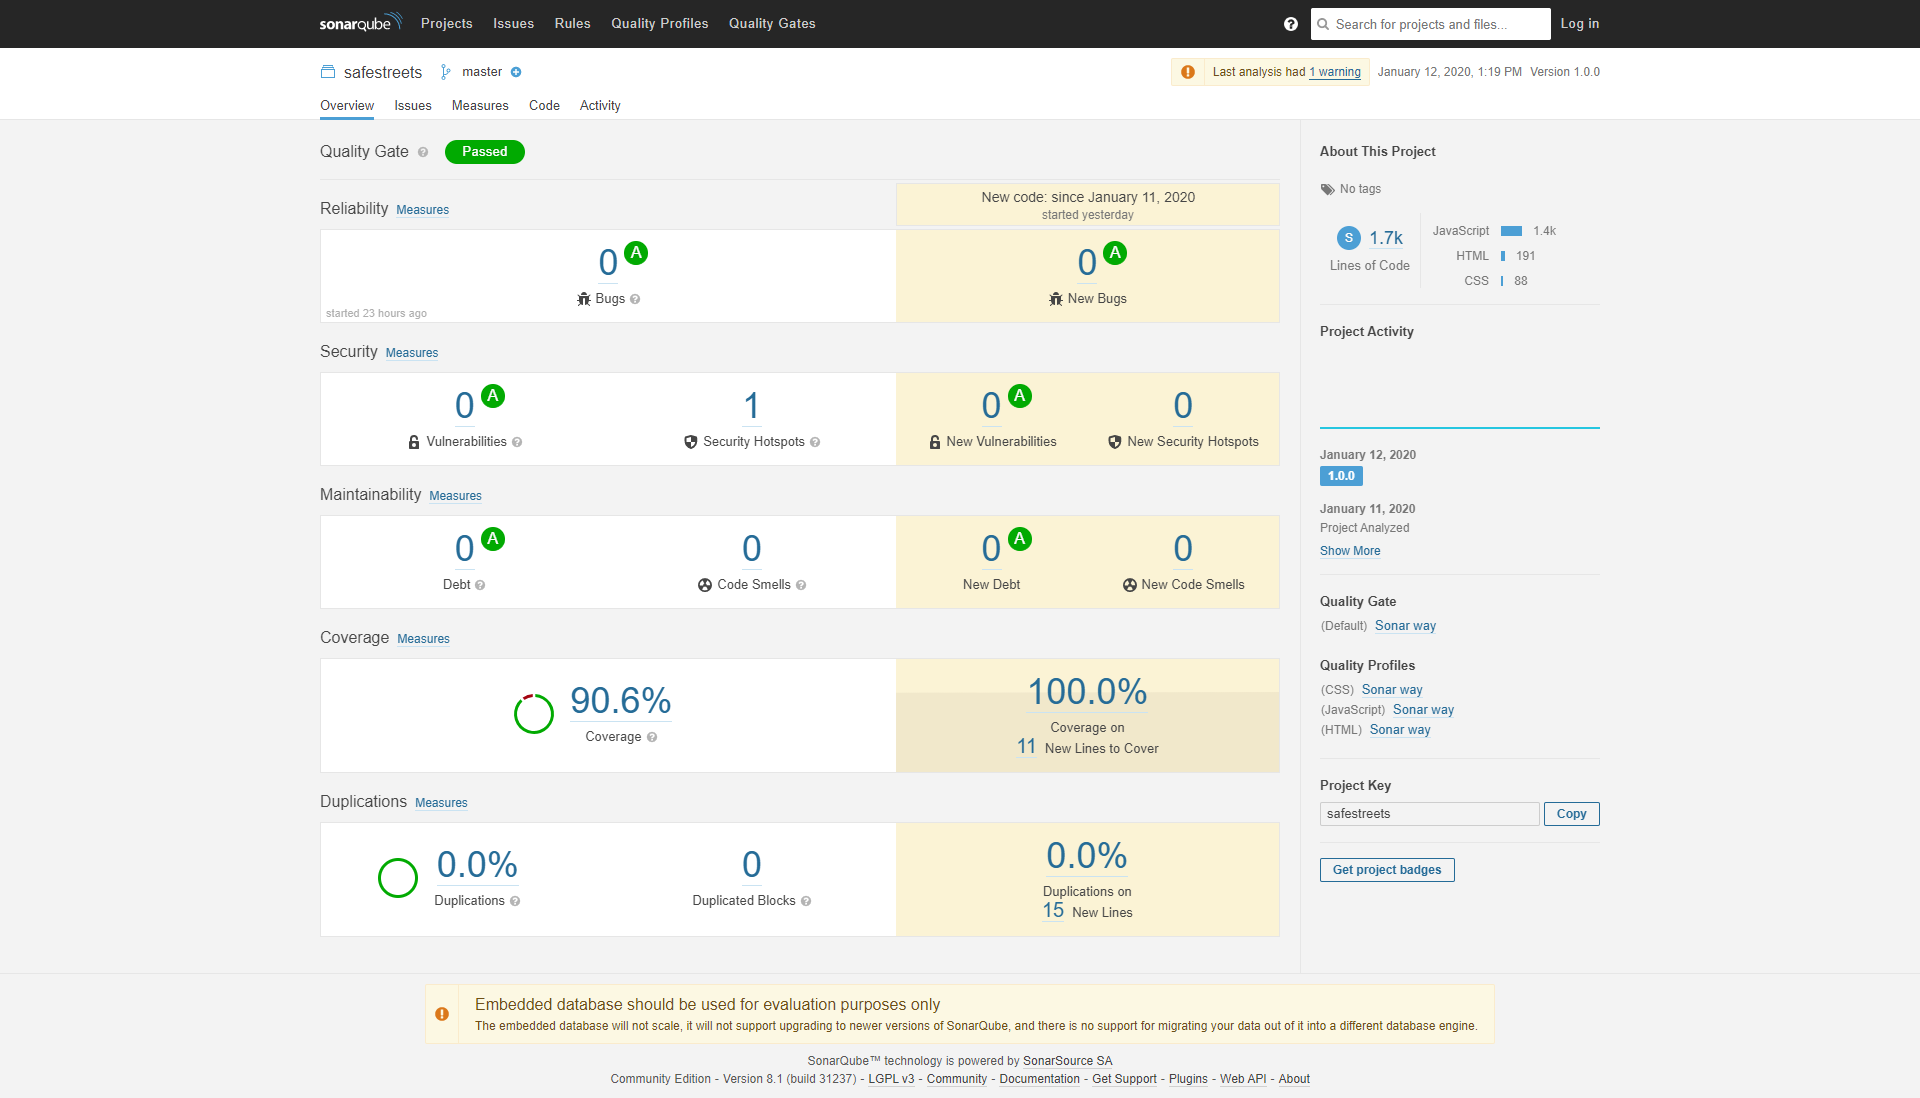
\includegraphics[width=1\linewidth]{Images/sonarReport}
	\caption{Sonar analysis results}
	\label{fig:sonarreport}
\end{figure}
